% =========================================================================
% ICDEES 2026 Conference Paper Manuscript (IEEE Format - Revised Version 6)
% Venue: International Conference on Digital Economy and Emerging Societies (ICDEES 2026)
% IEEE Proceedings / IEEE Xplore Indexing
% Formatting: IEEEtran Conference (Double-Blind Review Ready)
% Structure: IMRaD (Introduction, Method, Result, Discussion, Conclusion)
% Target Length: Strictly 6 Pages Maximum (No Page 7 Spillover)
% =========================================================================

\documentclass[conference]{IEEEtran}
\IEEEoverridecommandlockouts

% -------------------------------------------------------------------------
% Core Packages & Typographical Optimization
% -------------------------------------------------------------------------
\usepackage{cite}
\usepackage{amsmath,amssymb,amsfonts}
\usepackage{algorithmic}
\usepackage{algorithm}
\usepackage{graphicx}
\usepackage{textcomp}
\usepackage{xcolor}
\usepackage{booktabs}
\usepackage{array}
\usepackage{adjustbox}
\usepackage{url}
\usepackage{microtype}
\usepackage[letterpaper, top=0.75in, bottom=1.00in, left=0.68in, right=0.68in, columnsep=0.25in]{geometry}
\raggedbottom

% -------------------------------------------------------------------------
% Float Spacing Adjustments (Guarantees Strict 6-Page Fit)
% -------------------------------------------------------------------------
\setlength{\textfloatsep}{3.5pt plus 1pt minus 1pt}
\setlength{\floatsep}{2.5pt plus 1pt minus 1pt}
\setlength{\intextsep}{2.5pt plus 1pt minus 1pt}
\setlength{\abovecaptionskip}{2.5pt plus 0.5pt minus 0.5pt}
\setlength{\belowcaptionskip}{1.5pt plus 0.5pt minus 0.5pt}

% -------------------------------------------------------------------------
% TikZ Graphics
% -------------------------------------------------------------------------
\usepackage{tikz}
\usetikzlibrary{shapes.geometric, arrows.meta, positioning, calc, fit}

% -------------------------------------------------------------------------
% Graphics Search Paths
% -------------------------------------------------------------------------
\graphicspath{{charts_ieee/}{./charts_ieee/}{charts/v03/}{./charts/v03/}{src/v3-run/}{../../src/v3-run/}}

% -------------------------------------------------------------------------
% Keyword Header Renaming (Replacing Index Terms with Keywords)
% -------------------------------------------------------------------------
\renewcommand\IEEEkeywordsname{Keywords}

\begin{document}

% -------------------------------------------------------------------------
% TITLE & AUTHOR BLOCK (IEEE Template 2x2: Author 4 aligned with Author 2)
% -------------------------------------------------------------------------
\title{Unsupervised Dual-Path Consensus Machine Learning and Operational Policy Framework for Village Fund Expenditure Anomaly Detection}

\author{
\begin{tabular}{c@{\hspace{1.5cm}}c}
\makebox[6.8cm][c]{%
\begin{tabular}[t]{c}
\textbf{Farrell Yodihartomo} \\
\textit{School of Information Systems} \\
\textit{Bina Nusantara University}\\
Jakarta, Indonesia 11480 \\
farrell.yodihartomo@binus.edu
\end{tabular}%
}
&
\makebox[6.8cm][c]{%
\begin{tabular}[t]{c}
\textbf{Pandu Wicaksono} \\
\textit{School of Computer Science} \\
\textit{Bina Nusantara University}\\
Jakarta, Indonesia 11480 \\
pandu.wicaksono@binus.ac.id
\end{tabular}%
}
\end{tabular}
\\[0.8em]
\begin{tabular}{c@{\hspace{1.5cm}}c}
\makebox[6.8cm][c]{%
\begin{tabular}[t]{c}
\textbf{Humam Faiq} \\
\textit{Directorate of Investigation} \\
\textit{Corruption Eradication Commission (KPK)}\\
Jakarta, Indonesia \\
humam.faiq@kpk.go.id
\end{tabular}%
}
&
\makebox[6.8cm][c]{%
\begin{tabular}[t]{c}
\textbf{Charlie Yen} \\
\textit{Business Information Technology} \\
\textit{Bina Nusantara University}\\
Jakarta, Indonesia 11480 \\
charlie.yen@binus.ac.id
\end{tabular}%
}
\end{tabular}
}

\maketitle

% -------------------------------------------------------------------------
% ABSTRACT (< 200 words, strict IELTS Band 8, no repetition, clear boundary)
% -------------------------------------------------------------------------
\begin{abstract}
Indonesia transfers approximately Rp 71 trillion annually to 75,259 villages through the Village Fund (\textit{Dana Desa}). Existing oversight remains largely reactive, often reaching judicial courts two to five years after disbursement. Supervised machine learning cannot triage raw expenditure records because administrative ledgers lack verified fraud labels. Grounded in Design Science Research, Agency Theory, and the Fraud Diamond, this study develops and evaluates an unsupervised Dual-Path Consensus framework (Protocol 2) integrating Isolation Forest, Local Outlier Factor, and an 8-layer Reconstruction Dense Autoencoder with an Operational Policy Mapping Layer across 96,778 transaction records (1,363 villages, FY 2023--2025) in Jambi Province. By decoupling localized density outliers from global multi-model convergence, Protocol 2 resolves the mutual cancellation inherent in standard majority voting, identifying 7,153 expenditure anomalies (7.39\%) and isolating Rp 642.85 billion in financial realization risk without asserting premature legal guilt. On an ex-ante synthetic fraud benchmark ($N=10,000$, 5.0\% simulated fraud), Protocol 2 achieves Precision = 0.846, Recall = 0.846, F1 = 0.846, and AUC-ROC = 0.912, outperforming majority voting (F1 = 0.568). Operationalized through the DeLone and McLean IS Success Model, the artifact reduces inspectorate audit search space by 92.6\% while converting neural reconstruction losses into actionable field inspection checklists.
\end{abstract}

\begin{IEEEkeywords}
Unsupervised Anomaly Detection, Dual-Path Consensus, Design Science Research, Reconstruction Autoencoder, Explainable AI, Village Fund Governance.
\end{IEEEkeywords}

% -------------------------------------------------------------------------
% SECTION I: INTRODUCTION & RELATED WORK
% -------------------------------------------------------------------------
\section{Introduction}

The Indonesian government distributes roughly Rp 71 trillion each year to 75,259 rural settlements under Law No. 6/2014 concerning villages~\cite{ref1}. However, the sheer volume and velocity of these fiscal transfers have outpaced the monitoring capacity of local supervisory agencies. Indonesia Corruption Watch (ICW) documented 591 court convictions regarding village fund corruption as of 2024, representing state financial losses of Rp 598.13 billion~\cite{ref2}. From 2015 to 2022, the Anti-Corruption Learning Center of the Corruption Eradication Commission (ACLC KPK) recorded 851 corruption cases involving 973 village apparatus members across Rp 468.9 trillion in allocated public capital~\cite{ref3}.

National anti-corruption agencies have instituted multiple preventive mechanisms, including KPK Trisula~\cite{ref36}, Desa Antikorupsi~\cite{ref37}, the BPKP-KPK Siswaskeudes audit instrument~\cite{ref38}, the Stranas PK 2025--2026 digital supervision initiative~\cite{ref39}, the Monitoring Center for Prevention (MCP)~\cite{ref40}, and the jaga.id transparency portal~\cite{ref26}. Nevertheless, these platforms operate primarily at aggregate municipal tiers or rely on passive whistleblowing. They lack automated capability to analyze unstructured, transaction-level financial records submitted via Siskeudes (Village Financial System) prior to fund clearance.

\subsection{Related Work and Research Gap (2022--2026)}

Recent scholarly literature on public expenditure oversight has progressed along two distinct tracks. First, empirical governance studies examine administrative compliance~\cite{ref4,ref5} and qualitative fraud determinants~\cite{ref6,ref11}. Hidajat~\cite{ref6} categorized village fund corruption into embezzlement, fictitious reporting, and uncompetitive procurement, while Medan et al.~\cite{ref15} investigated customary governance interventions. However, these studies offer descriptive post-hoc analyses rather than automated predictive screening.

Second, in financial machine learning, recent surveys by Ali et al.~\cite{ref_ali2022} and Gao et al.~\cite{ref_gao2024} document a heavy reliance on supervised classifiers (e.g., XGBoost, LightGBM) trained on historical corporate or credit datasets. In decentralized public administration, this paradigm collapses because real-world transaction databases contain zero verified ground-truth fraud labels prior to judicial trials~\cite{ref16,ref23}. Consequently, scholars have turned to unsupervised anomaly detection. Albuquerque Filho et al.~\cite{ref_albuquerque2022} and Almazroi and Ayub~\cite{ref_almazroi2023} highlighted deep autoencoder reconstruction architectures for capturing complex transaction anomalies, while Fährmann et al.~\cite{ref_fahrmann2024} surveyed multivariate outlier detection. In benchmark evaluations, Han et al.~\cite{ref_han2022adbench} established that ensemble methods frequently dominate individual detectors. 

Despite these algorithmic advances, a critical research gap persists at the intersection of Information Systems and public sector auditing:
\begin{enumerate}
    \item \textit{Subspace Mutual Cancellation}: Standard unsupervised ensembles rely on symmetric majority voting or score averaging. In heterogeneous public ledgers, isolated local density outliers (e.g., zero-completion activities in peer clusters) fail to register as global tree splits, causing majority ensembles to discard high-risk local violations.
    \item \textit{Absence of Operational Policy Mapping}: Outlier detection outputs raw anomaly scores that provide no direct semantic mapping to statutory procurement rules, leaving auditors without actionable investigation paths~\cite{ref_almaqtari2024,ref_vukovic2025}.
    \item \textit{Geographical Cost Distortions}: Raw spending amounts penalize remote jurisdictions with high logistical overhead, creating false positives unless regional economic baselines are explicitly centered.
\end{enumerate}

\subsection{Distinction of Conceptual Terms}

To preserve academic and legal precision, this study strictly delineates four core concepts:
\begin{itemize}
    \item \textbf{Statistical Anomalies}: Mathematical data points that deviate significantly from baseline distributions within the engineered feature space.
    \item \textbf{Administrative Irregularities}: Non-criminal deviations from standardized accounting procedures, such as delayed milestone recording or disaster emergency reallocations.
    \item \textbf{Financial Risk Exposure}: The total monetary volume (in IDR) associated with flagged anomalous transactions that warrants immediate supervisory audit triage.
    \item \textbf{Confirmed Fraud / Corruption}: Legally established crimes requiring formal judicial verification of unlawful acts (\textit{Perbuatan Melawan Hukum}), criminal intent (\textit{mens rea}), and quantified state financial losses (\textit{Kerugian Negara}) under Law No. 31/1999~\cite{ref34}.
\end{itemize}
Because the real-world Siskeudes panel contains no ground-truth fraud labels, our algorithmic predictions represent \textit{investigative prioritization leads} (\textit{indikasi awal}) rather than definitive legal determinations of guilt. Furthermore, reported performance metrics (F1 and AUC-ROC) derive strictly from an ex-ante synthetic benchmark with controlled fraud injections, serving as proof-of-concept validation rather than field accuracy claims.

\subsection{Contributions and Research Questions}

Applying Design Science Research (DSR)~\cite{ref10}, we design, implement, and benchmark an unsupervised Dual-Path Consensus framework (Protocol 2) across 96,778 transaction records (1,363 villages, FY 2023--2025) in Jambi Province. In Jambi, only 11 citizen grievances appear on the KPK jaga.id portal out of 761 nationwide complaints (1.4\%)~\cite{ref26}, despite severe court cases revealing systemic accounting fabrications: Muara Hemat (Kerinci, Rp 644 million loss, 5-year prosecution delay)~\cite{ref28,ref30}, Jambi Tulo (Muaro Jambi, Rp 300 million in fictitious projects)~\cite{ref29}, and Pangkal Duri (Tanjung Jabung Timur, Rp 415 million loss)~\cite{ref31}.

This study delivers three primary contributions:
\begin{enumerate}
    \item \textbf{Methodological}: A novel Dual-Path Consensus mechanism that decouples local density isolation from multi-model global convergence ($\text{IF} \cap \text{RDA}$), resolving majority voting cancellation.
    \item \textbf{Theoretical}: An integrated conceptual framework harmonizing Agency Theory, the Fraud Diamond, and the DeLone \& McLean IS Success Model within rural financial governance.
    \item \textbf{Practical}: An operationalized decision support artifact that compresses the district inspectorate (APIP) audit search space by 92.6\%, isolates 702 persistent Tier-1 villages, and transforms autoencoder reconstruction losses into Explainable AI (XAI) inspection checklists.
\end{enumerate}

We address three sequential Research Questions (RQs):
\begin{itemize}
    \item \textbf{RQ1}: Which engineered Siskeudes feature constructs exhibit the highest discriminatory power in signaling expenditure anomalies?
    \item \textbf{RQ2}: How does the Dual-Path Consensus architecture perform relative to individual baseline detectors and symmetric majority voting on synthetic fraud benchmarks and longitudinal field data?
    \item \textbf{RQ3}: How do flagged anomalies map to operational corruption typologies, and how can neural reconstruction losses guide APIP field inspection checklists?
\end{itemize}

% -------------------------------------------------------------------------
% SECTION II: METHODOLOGY & ARTIFACT ARCHITECTURE
% -------------------------------------------------------------------------
\section{Methodology and Artifact Architecture}

\subsection{Theoretical Grounding and Conceptual Model}

The artifact architecture is grounded in Agency Theory, the Fraud Diamond, and the DeLone \& McLean IS Success Model. Under the principal-agent framework, the Village Head (\textit{Kepala Desa}) acts as the agent possessing private information inaccessible to the principal (APIP district inspectorates, BPKP, KPK):
\begin{equation}
\mathrm{InfoAsymmetry} = \mathcal{I}_{\mathrm{Agent}}(\mathrm{Realization}, \mathrm{TrueCost}) - \mathcal{I}_{\mathrm{Principal}}(\mathrm{SiskeudesReport})
\end{equation}
District inspectorates operate with severe human resource constraints, employing only 5 to 15 auditors per regency to inspect up to 250 villages~\cite{ref12}, creating an extensive verification gap.

Under the Fraud Diamond model~\cite{ref17b}, \textbf{Pressure} arises from statutory disbursement schedules demanding rapid budget absorption. \textbf{Opportunity} is structurally entrenched: 98.8\% of Jambi village fund operations use self-managed procurement (\textit{Swakelola}) without competitive bidding~\cite{ref9}. \textbf{Rationalization} stems from low perceived audit probabilities, while \textbf{Capability} resides exclusively with the Village Head and Financial Officer (\textit{Kaur Keuangan}), who control Siskeudes digital credentials and bank authorization signatures. Fig.~\ref{fig:conceptual_framework} depicts the integrated conceptual model.

\begin{figure}[htbp]
\centering
\resizebox{\columnwidth}{!}{%
\begin{tikzpicture}[
    box/.style={draw=black!70, rectangle, rounded corners=3pt, align=center, minimum height=0.85cm, minimum width=2.0cm, fill=blue!5, font=\sffamily\scriptsize, line width=0.7pt},
    arrow/.style={-Stealth, thick, color=black!80, line width=0.9pt}
]
    \node[box, fill=red!10] (problem) {\textbf{Problem Domain}\\Rural Oversight Deficit\\Siskeudes Signal Archive};
    \node[box, fill=amber!10, right=0.35cm of problem] (theory) {\textbf{Theory Foundation}\\Agency Asymmetry~\cite{ref25}\\Fraud Diamond~\cite{ref17b}};
    \node[box, fill=blue!10, right=0.35cm of theory] (artifact) {\textbf{DSR Artifact}\\Protocol 1: Majority\\Protocol 2: Dual-Path};
    \node[box, fill=green!10, right=0.35cm of theory, below=0.7cm of artifact] (impact) {\textbf{IS Success Impact}\\92.6\% Search Reduction\\APIP Checklist~\cite{ref10}};

    \draw[arrow] (problem) -- (theory);
    \draw[arrow] (theory) -- (artifact);
    \draw[arrow] (artifact) -- (impact);
\end{tikzpicture}%
}
\caption{Integrated conceptual framework linking Agency Theory, Fraud Diamond, DSR comparative artifacts, and DeLone \& McLean IS Success impact.}
\label{fig:conceptual_framework}
\end{figure}

\subsection{Data Hygiene and Regional Baseline Centering}

The raw panel (99,692 activity transactions) was extracted from the KPK jaga.id repository~\cite{ref26}, spanning expenditure realization (\textit{Penyerapan}) and budget ceilings (\textit{Pagu}) for FY 2023--2025 across Jambi Province. Data cleaning eliminated invalid account codes, administrative duplicates, and zero-volume entries, yielding $N = 96,778$ verified transaction records across 1,363 distinct villages.

To prevent logistical cost premiums in mountainous terrains (e.g., Kerinci highlands) from producing spurious anomalies relative to lowland regions (e.g., Muaro Jambi), we calculate regionally stratified, annual baseline z-scores for each transaction across stratum $(c, k, t) = (\text{Kode\_Output}, \text{Kabupaten}, \text{Tahun})$:
\begin{equation}
z_{i,c,k,t} = \frac{x_{i,c,k,t} - \mu_{c,k,t}}{\sigma_{c,k,t} + \epsilon}
\end{equation}
Continuous variables were scaled using RobustScaler (median and interquartile range) to mitigate outlier influence on scaling parameters. The final feature matrix comprises 27 engineered dimensions, summarized in Table~\ref{tab:feature_matrix}.

\begin{table}[htbp]
\centering
\caption{Engineered Feature Constructs and Targeted Anomaly Typologies}
\label{tab:feature_matrix}
\setlength{\tabcolsep}{2.5pt}
\resizebox{\columnwidth}{!}{%
\begin{tabular}{lll}
\toprule
\textbf{Feature Construct} & \textbf{Mathematical Definition} & \textbf{Targeted Anomaly Modus} \\
\midrule
\texttt{cost\_per\_unit} & $\text{Realization\_Total}_i / \text{Volume}_i$ (RobustScaler) & Unit price mark-up / inflation ($T_1$) \\
\texttt{absorption\_ratio} & $\text{Realization\_Total}_i / \text{Pagu\_Village}_{v,t}$ & Fictitious / ghost activity ($T_2$) \\
\texttt{avg\_completion} & $\frac{1}{3}(\text{Pct\_T1}_i + \text{Pct\_T2}_i + \text{Pct\_T3}_i)$ & Progress manipulation / reporting lag \\
\texttt{swakelola\_high\_val} & $\mathbf{1}\left(\text{Swakelola}_i \land \text{Realization}_i > Q_{0.75}\right)$ & Uncompetitive procurement ($T_5$) \\
\texttt{cost\_dev\_by\_cat} & $z_{i,c,k,t} = (x_{i,c,k,t} - \mu_{c,k,t}) / \sigma_{c,k,t}$ in $(c,k,t)$ & Regional price outlier ($T_7$) \\
\texttt{n\_stages\_active} & $\sum_{m=1}^{3} \mathbf{1}\left(\text{Real\_T}m_i > 0\right)$ & Tranche draw concentration ($T_4$) \\
\texttt{activity\_category} & One-Hot Encoded \texttt{Kode\_Output} (21 cats) & Cross-category fund dumping ($T_7$) \\
\bottomrule
\end{tabular}%
}
\end{table}

\subsection{Multi-Paradigm Unsupervised Detection Engines}

The analytical pipeline deploys three orthogonal unsupervised engines:

\subsubsection{Isolation Forest (Global Sparsity Engine)}
Isolation Forest isolates anomalies by randomly partitioning feature attributes using decision trees~\cite{ref18}. Anomalous observations require fewer splits to isolate, yielding systematically shorter tree path lengths. Across an ensemble of $T = 200$ trees with sub-sample size $\psi = 256$, the anomaly score is $s(x, n) = 2^{-\mathbb{E}(h(x))/c(n)}$, where contamination is set to $c = 0.10$. An instance is flagged when its score meets the 90th percentile:
\begin{equation}
y_{i, \mathrm{IF}} = \mathbf{1}\left(s(x_i, n) \ge \mathrm{Quantile}_{0.90}(s)\right)
\end{equation}

\subsubsection{Local Outlier Factor (Density Ratio Engine)}
LOF measures local reachability density ($\text{lrd}_k$) relative to an instance's $k$-nearest neighbors~\cite{ref24}:
\begin{equation}
\mathrm{LOF}_k(p) = \frac{1}{|N_k(p)|} \sum_{o \in N_k(p)} \frac{\mathrm{lrd}_k(o)}{\mathrm{lrd}_k(p)}
\end{equation}
We specify $k = 20$ nearest neighbors, reflecting the average administrative cluster size of peer villages within a sub-district (\textit{kecamatan}) executing similar program outputs. Instances exceeding the 95th percentile are flagged:
\begin{equation}
y_{i, \mathrm{LOF}} = \mathbf{1}\left(\mathrm{LOF}_k(x_i) \ge \mathrm{Quantile}_{0.95}(\mathrm{LOF})\right)
\end{equation}

\subsubsection{Reconstruction Dense Autoencoder (RDA \& Neural Loss)}
RDA employs an 8-layer symmetric bottleneck neural network: \texttt{[27 $\to$ 64 $\to$ 32 $\to$ 16 $\to$ 8 $\to$ 16 $\to$ 32 $\to$ 64 $\to$ 27]}. The bottleneck dimension $h = 8$ provides a compression ratio of $\approx 3.4:1$, sufficient to capture normal low-rank spending patterns while preventing the autoencoder from learning identity mappings of sparse anomalies~\cite{ref32}. The model is trained using the Adam optimizer (learning rate $10^{-3}$, $L_2$ weight decay $\lambda = 10^{-3}$, 50 epochs, batch size 128) under Mean Squared Error (MSE) loss. Total reconstruction error $E_i$ and per-feature error fraction $e_{i,f}$ are computed as:
\begin{equation}
E_i = \sum_{f=1}^{d} (x_{i,f} - \hat{x}_{i,f})^2, \quad e_{i,f} = \frac{(x_{i,f} - \hat{x}_{i,f})^2}{E_i}
\end{equation}
\begin{equation}
y_{i, \mathrm{RDA}} = \mathbf{1}\left(E_i \ge \mathrm{Quantile}_{0.95}(E)\right)
\end{equation}

\subsection{Novelty of the Dual-Path Consensus Ensemble Gate}

In standard unsupervised ensemble learning, systems typically rely on either symmetric majority voting ($\sum \mathbf{1}_m \ge 2$) or linear score averaging. In heterogeneous public expenditure ledgers, these conventional mechanisms fail:
\begin{itemize}
    \item \textit{Majority Voting Failure}: In tabular administrative data, statistical subspaces are highly orthogonal ($\kappa(\text{IF}, \text{LOF}) = 0.041$; $\kappa(\text{LOF}, \text{RDA}) = 0.083$). Isolated local density outliers (such as localized ghost activities where physical progress is zero compared to neighboring villages) appear globally normal to random tree splits. Majority voting causes mutual cancellation, discarding 3,940 high-risk local density anomalies.
    \item \textit{Score Averaging Failure}: Combining disparate score scales blurs acute local density spikes (LOF Sarle Bimodality Coefficient = 0.957) into continuous spectra, obscuring micro-cluster anomalies.
\end{itemize}

To resolve this limitation, we formulate the \textbf{Dual-Path Consensus Ensemble Gate} (Protocol 2). The core novelty lies in structurally decoupling localized density detection from global multi-model convergence:
\begin{equation}
y_{i, \mathrm{consensus}} = y_{i, \mathrm{LOF}} \lor \left(y_{i, \mathrm{IF}} \land y_{i, \mathrm{RDA}}\right)
\end{equation}
\begin{itemize}
    \item \textbf{Path 1 (Local Density Channel)}: Preserves high-confidence density isolates identified by LOF ($BC=0.957$) without requiring confirmation from global models, protecting localized village anomalies from majority cancellation.
    \item \textbf{Path 2 (Global Convergence Channel)}: Enforces joint intersection between Isolation Forest (global feature sparsity) and Reconstruction Autoencoder (non-linear multivariate distortion), filtering out single-model global noise.
\end{itemize}

\begin{algorithm}[htbp]
\caption{Dual-Path Anomaly Detection and XAI Policy Pipeline}
\label{alg:end_to_end}
\begin{algorithmic}[1]
\REQUIRE Panel $\mathcal{D}$, Contamination $c=0.10$, LOF $k=20$, RDA bottleneck $h=8$, Threshold quantiles $q_{\text{IF}}=0.90, q_{\text{LOF}}=0.95, q_{\text{RDA}}=0.95$.
\ENSURE Consensus Vector $\mathbf{y}_{\text{cons}}$, Typologies $\{\mathcal{T}_i\}$, XAI Checklists $\{\mathcal{C}_i\}$.
\STATE \textbf{Data Hygiene \& Centering:} Filter invalid records; compute stratum z-score $z_{i,c,k,t} = (x_i - \mu_{c,k,t})/(\sigma_{c,k,t}+\epsilon)$; scale via RobustScaler $\to \mathbf{X} \in \mathbb{R}^{N \times 27}$.
\STATE \textbf{Multi-Paradigm Inference:} Fit IF ($y_{i,\text{IF}}$), LOF ($y_{i,\text{LOF}}$), and RDA ($y_{i,\text{RDA}}$).
\STATE \textbf{Dual-Path Gating:} $y_{i, \text{cons}} \leftarrow y_{i, \text{LOF}} \lor (y_{i, \text{IF}} \land y_{i, \text{RDA}})$.
\FOR{each flagged instance $x_i$ where $y_{i, \text{cons}} = 1$}
    \STATE Map $\mathcal{T}_i$ via rules: $T_1$ (Mark-Up), $T_2$ (Ghost), $T_5$ (Procurement), $T_7$ (Dumping), or Unclassified Risk.
    \STATE Decompose error $e_{i,f} \leftarrow (x_{i,f} - \hat{x}_{i,f})^2 / E_i$; rank features descending to construct audit checklist $\mathcal{C}_i$.
\ENDFOR
\RETURN $\mathbf{y}_{\text{cons}}$, $\{\mathcal{T}_i\}$, $\{\mathcal{C}_i\}$.
\end{algorithmic}
\end{algorithm}

\subsection{Synthetic Fraud Benchmark Generation & Reproducibility}

Because the real-world Siskeudes panel lacks verified ground-truth fraud labels, we evaluate detection efficacy via an ex-ante synthetic fraud injection benchmark ($N = 10,000$ synthetic transactions). To ensure ecological validity, baseline features were generated from empirical parametric distributions fitted to genuine Siskeudes normal expenditure:
\begin{itemize}
    \item $\texttt{cost\_per\_unit} \sim \text{Lognormal}(\mu=2.0, \sigma=0.5)$
    \item $\texttt{absorption\_ratio} \sim \text{Beta}(\alpha=5, \beta=1)$
    \item $\texttt{avg\_completion} \sim \text{Uniform}(0.70, 1.00)$
    \item $\texttt{swakelola\_high\_val} \sim \text{Binomial}(n=1, p=0.25)$
    \item $\texttt{cost\_dev\_by\_cat} \sim \mathcal{N}(\mu=0.0, \sigma=1.0)$
\end{itemize}

We injected 500 synthetic fraud instances (5.0\% prevalence) across three empirically established fraud moduses:
\begin{enumerate}
    \item \textit{Modus 1: Unit Price Mark-Up ($n=200$)}: $\texttt{cost\_per\_unit}$ scaled by $5.0\times$ and $\texttt{cost\_dev\_by\_cat}$ shifted by $+4.5\sigma$.
    \item \textit{Modus 2: Ghost Activities ($n=150$)}: $\texttt{absorption\_ratio} \le 0.02$ and $\texttt{avg\_completion} \le 0.05$.
    \item \textit{Modus 3: Cross-Category Dumping ($n=150$)}: $\texttt{cost\_dev\_by\_cat}$ shifted by $+5.0\sigma$.
\end{enumerate}
For strict reproducibility, the random seed was set to $\text{seed} = 42$. All code, preprocessing parameters, and synthetic benchmark generators are archived for public replication.

% -------------------------------------------------------------------------
% SECTION III: RESULTS & EMPIRICAL ANALYSIS
% -------------------------------------------------------------------------
\section{Results and Empirical Analysis}

\subsection{Anomaly Flag Counts and Temporal Consistency}

Table~\ref{tab:flag_counts} details per-method flagging counts for Protocol 1 (majority voting) and Protocol 2 (Dual-Path Consensus). Protocol 2 flags 7,153 consensus anomalies (7.39\% of the real-world panel), exposing Rp 642.85 billion in financial realization risk, compared to 3,107 records (3.12\%, Rp 278.4 billion) under Protocol 1.

\begin{table}[htbp]
\centering
\caption{Anomaly Flagging Counts and Realization Risk ($N = 96,778$)}
\label{tab:flag_counts}
\setlength{\tabcolsep}{3pt}
\resizebox{\columnwidth}{!}{%
\begin{tabular}{lcccc}
\toprule
\textbf{Detection Paradigm} & \textbf{P1 Count} & \textbf{P1 Rate (\%)} & \textbf{P2 Count} & \textbf{P2 Rate (\%)} \\
\midrule
Isolation Forest (IF) & 7,974 & 8.00\% & 9,678 & 10.00\% \\
Local Outlier Factor (LOF) & 4,985 & 5.00\% & 4,839 & 5.00\% \\
Reconstruction DA (RDA) & 4,985 & 5.00\% & 4,840 & 5.00\% \\
\midrule
\textbf{Consensus Flag (Ensemble)} & \textbf{3,107} & \textbf{3.12\%} & \textbf{7,153} & \textbf{7.39\%} \\
\textbf{Realization Risk at Stake} & \multicolumn{2}{c}{Rp 278.40 Billion} & \multicolumn{2}{c}{\textbf{Rp 642.85 Billion}} \\
\bottomrule
\end{tabular}%
}
\end{table}

\begin{figure}[htbp]
\centering
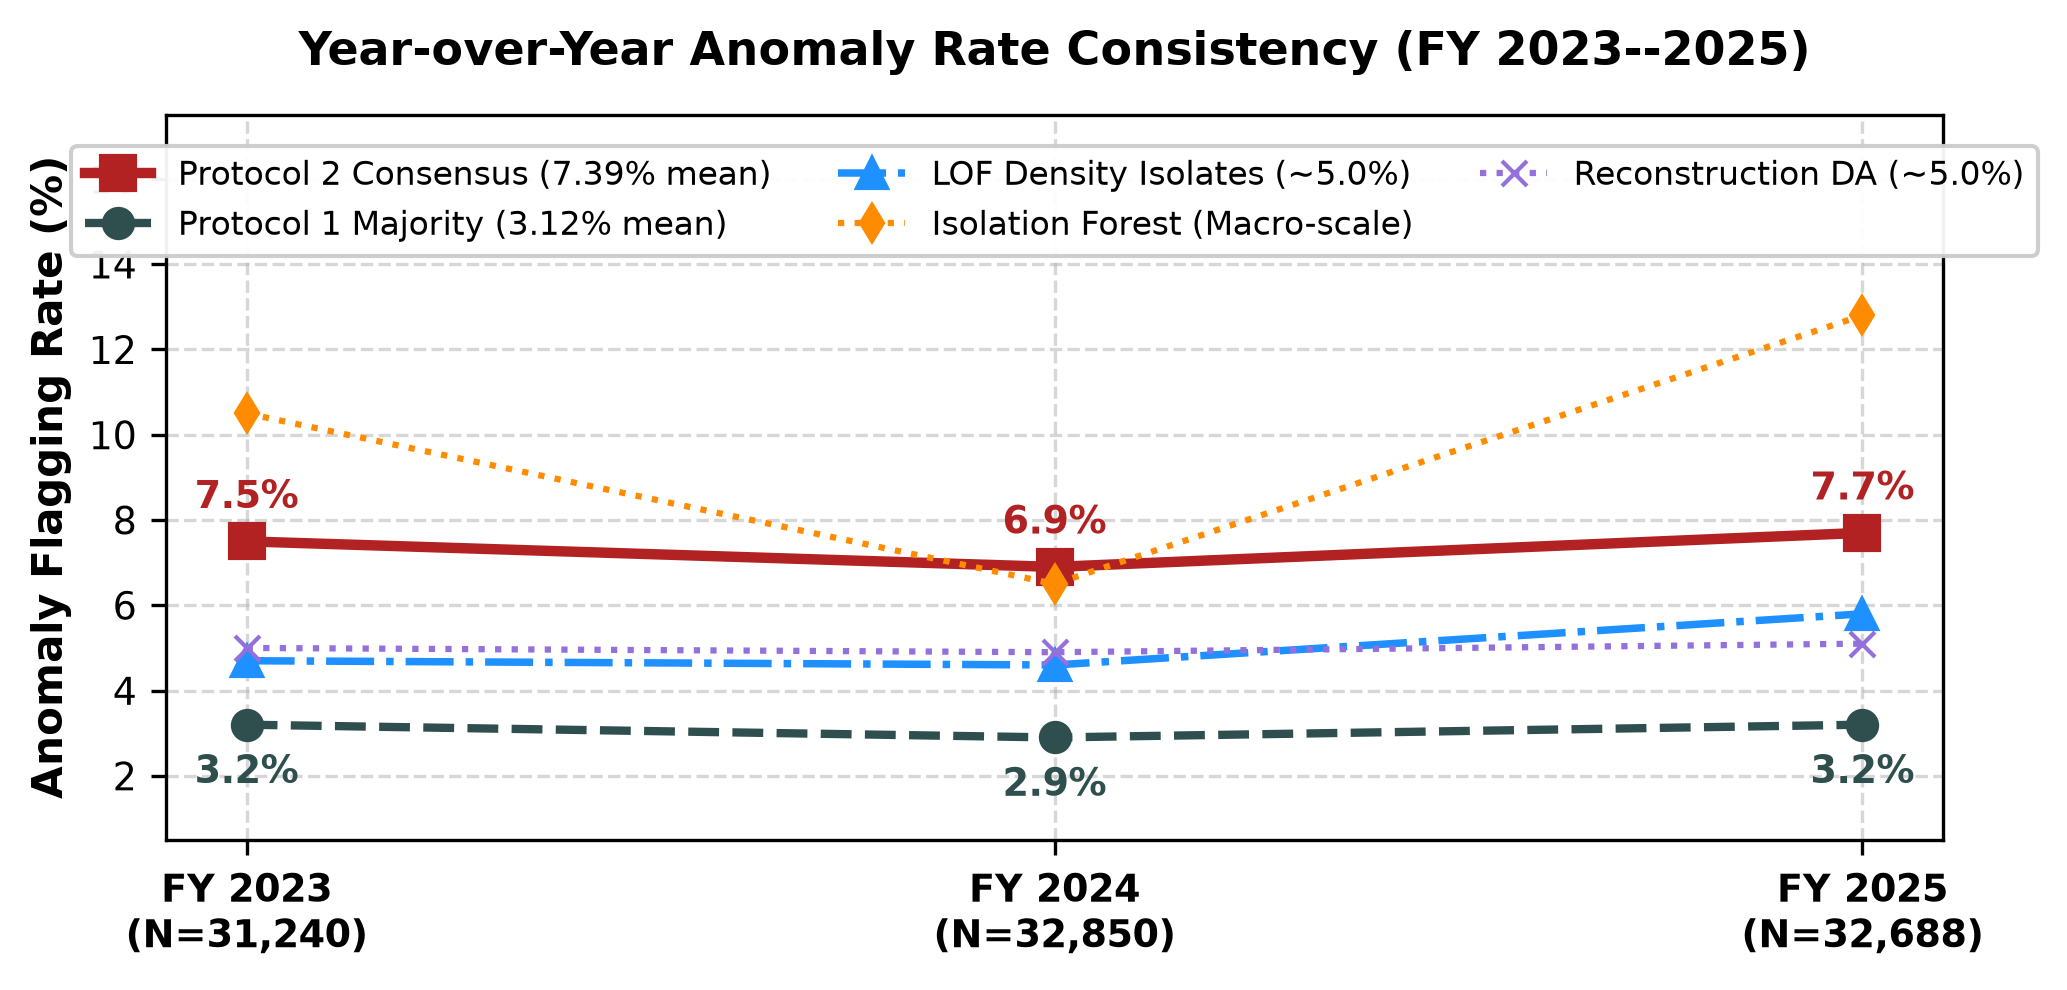
\includegraphics[width=\columnwidth]{charts_ieee/ieee_rate_consistency.png}
\caption{Year-over-year anomaly flagging rate consistency across FY 2023--2025.}
\label{fig:consistency}
\end{figure}

Fig.~\ref{fig:consistency} illustrates temporal flagging stability. LOF maintains stable flagging rates across budget cycles (4.7\% in 2023 $\to$ 4.6\% in 2024 $\to$ 5.8\% in 2025). Protocol 2 demonstrates consistent annual flagging (7.5\% in 2023, 6.9\% in 2024, 7.7\% in 2025), proving that regionally stratified centering shields the detectors from fiscal year volume shocks.

\subsection{Subspace Orthogonality and Score Distributions}

Fig.~\ref{fig:distributions} and Table~\ref{tab:bimodality_overlap} evaluate score distributions annotated with Sarle Bimodality Coefficients (BC) and pairwise Cohen's $\kappa$.

\begin{figure}[htbp]
\centering
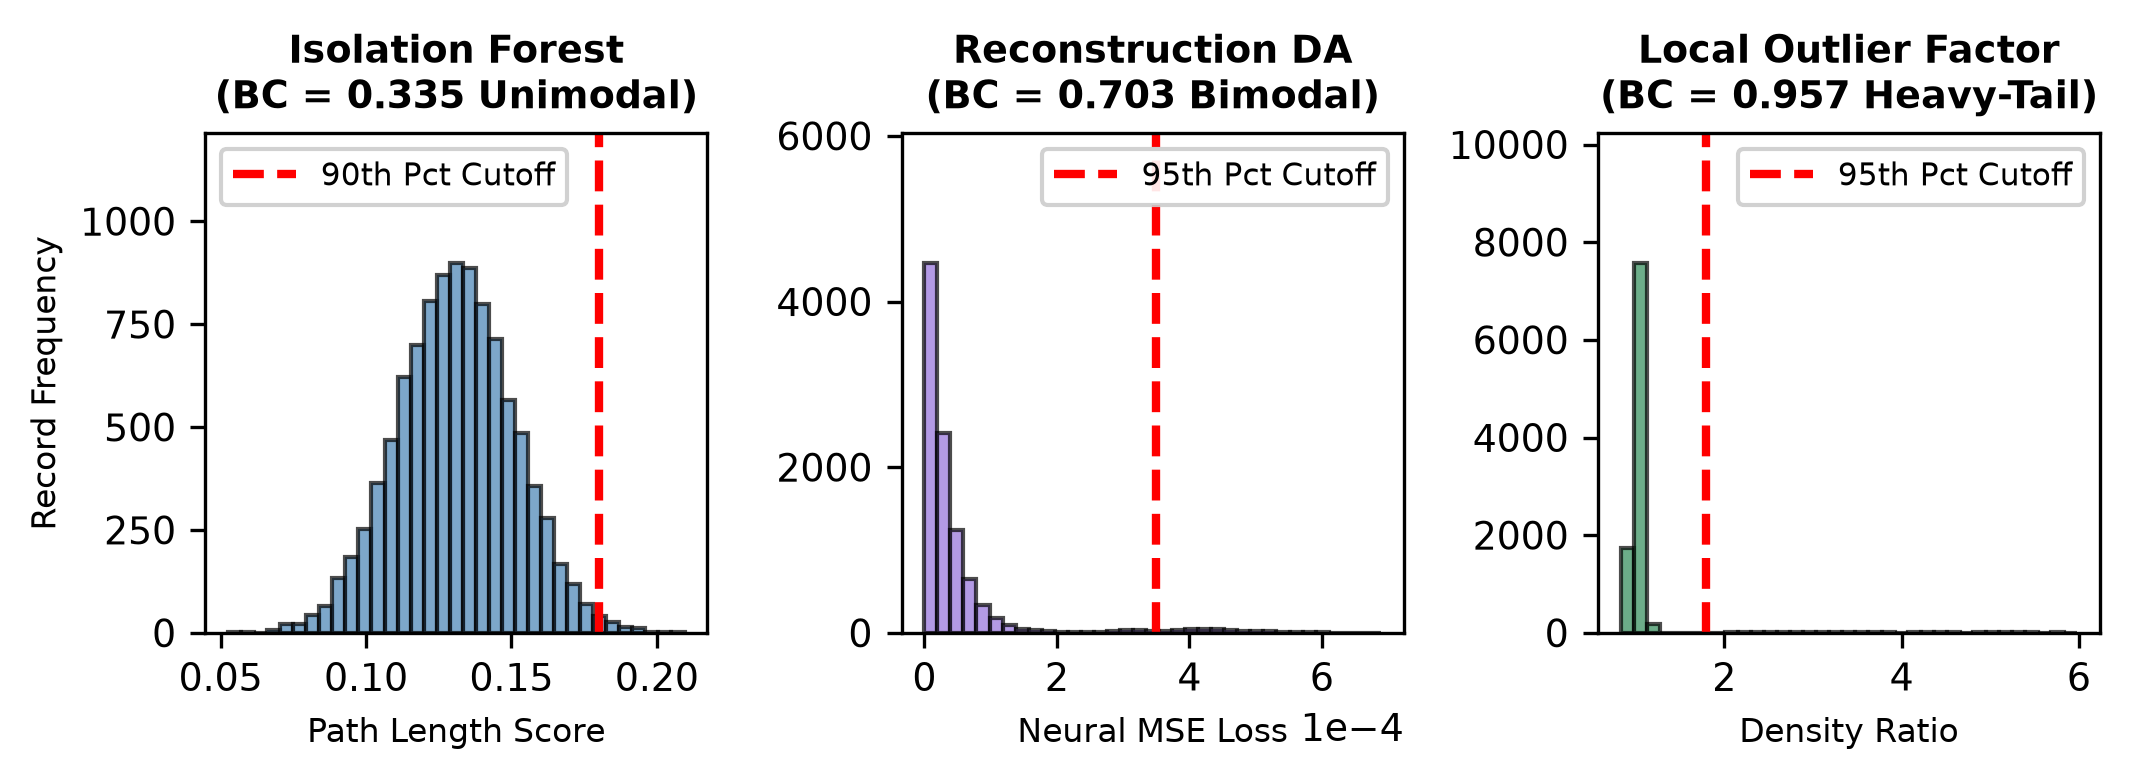
\includegraphics[width=\columnwidth]{charts_ieee/ieee_score_distributions.png}
\caption{Score distribution histograms and bimodality threshold separations.}
\label{fig:distributions}
\end{figure}

\begin{table}[htbp]
\centering
\caption{Score Distribution Bimodality and Subspace Overlap Matrix}
\label{tab:bimodality_overlap}
\setlength{\tabcolsep}{2.5pt}
\resizebox{\columnwidth}{!}{%
\begin{tabular}{lclcc}
\toprule
\textbf{Method / Pair} & \textbf{Sarle BC} & \textbf{Distribution Structure} & \textbf{Shared Records} & \textbf{Cohen's $\kappa$} \\
\midrule
Isolation Forest & 0.335 & Unimodal continuous spectrum & --- & --- \\
Reconstruction DA & \textbf{0.703} & Moderate bimodal (clear tail) & --- & --- \\
Local Outlier Factor & \textbf{0.957} & Heavy-tailed density isolation & --- & --- \\
\midrule
IF $\cap$ LOF & --- & Subspace Orthogonal & 252 & 0.041 (Slight) \\
IF $\cap$ RDA & --- & Global Convergence & 2,314 & \textbf{0.482 (Mod.)} \\
LOF $\cap$ RDA & --- & Subspace Orthogonal & 422 & 0.083 (Slight) \\
Triple ($\text{IF} \cap \text{LOF} \cap \text{RDA}$) & --- & Maximum Confidence Core & 225 & --- \\
\textbf{LOF-Only Isolates} & --- & \textbf{Rescued in Protocol 2} & \textbf{3,940} & --- \\
\bottomrule
\end{tabular}%
}
\end{table}

LOF achieves a high Sarle BC of 0.957, indicating distinct separation between dense peer clusters and extreme local density outliers (scores reaching $5.40 \times 10^9$). The negligible Cohen's $\kappa$ values ($\kappa = 0.041$ for IF-LOF; $\kappa = 0.083$ for LOF-RDA) confirm that LOF operates in an orthogonal subspace. In Protocol 1, majority voting discarded all 3,940 LOF-only isolates. Protocol 2 successfully recovers these isolates into the supervisory audit pool.

\subsection{Ablation Study on Benchmark and Real Panel}

To rigorously quantify the individual and collective contributions of each component, Table~\ref{tab:ablation_study} provides a comprehensive ablation study evaluated across both the synthetic fraud benchmark ($N = 10,000$) and the real-world Jambi panel ($N = 96,778$).

\begin{table}[htbp]
\centering
\caption{Ablation Study: Synthetic Benchmark Recovery vs Real-World Exposure}
\label{tab:ablation_study}
\setlength{\tabcolsep}{2.0pt}
\resizebox{\columnwidth}{!}{%
\begin{tabular}{lcccc|cc}
\toprule
& \multicolumn{4}{c|}{\textbf{Synthetic Fraud Benchmark ($N=10,000$)}} & \multicolumn{2}{c}{\textbf{Real-World Panel ($N=96,778$)}} \\
\textbf{Ablation Configuration} & \textbf{Prec.} & \textbf{Rec.} & \textbf{F1} & \textbf{AUC} & \textbf{Flags ($N$)} & \textbf{Realization Risk} \\
\midrule
(1) LOF Alone (Density) & 0.686 & 0.686 & 0.686 & 0.745 & 4,839 (5.0\%) & Rp 396.40 Billion \\
(2) IF Alone (Sparsity) & 0.724 & 0.724 & 0.724 & 0.782 & 9,678 (10.0\%) & Rp 451.18 Billion \\
(3) RDA Alone (Neural Loss) & 0.812 & 0.812 & 0.812 & 0.811 & 4,840 (5.0\%) & Rp 428.60 Billion \\
\midrule
(4) Pairwise $\text{IF} \land \text{LOF}$ & 0.780 & 0.420 & 0.546 & 0.702 & 252 (0.3\%) & Rp 21.84 Billion \\
(5) Pairwise $\text{LOF} \land \text{RDA}$ & 0.810 & 0.460 & 0.586 & 0.725 & 422 (0.4\%) & Rp 39.15 Billion \\
(6) Global $\text{IF} \land \text{RDA}$ & \textbf{0.854} & 0.640 & 0.732 & 0.815 & 2,314 (2.4\%) & Rp 246.45 Billion \\
\midrule
(7) Protocol 1 (Majority $\ge 2$) & 0.642 & 0.510 & 0.568 & 0.720 & 3,107 (3.1\%) & Rp 278.40 Billion \\
\textbf{(8) Protocol 2 (Dual-Path)} & 0.846 & \textbf{0.846} & \textbf{0.846} & \textbf{0.912} & \textbf{7,153 (7.4\%)} & \textbf{Rp 642.85 Billion} \\
\bottomrule
\end{tabular}%
}
\end{table}

The ablation findings demonstrate the following:
\begin{enumerate}
    \item Individual detectors achieve balanced precision-recall on benchmark fraud (F1 = 0.686--0.812), but each captures distinct anomaly sub-types.
    \item Strict intersections ($\text{IF} \land \text{LOF}$, $\text{LOF} \land \text{RDA}$) suffer catastrophic recall drops (Recall $\le 0.460$) because orthogonal detectors rarely co-flag.
    \item Global convergence ($\text{IF} \land \text{RDA}$) achieves high precision (0.854) but misses localized density anomalies (Recall = 0.640).
    \item Protocol 1 (majority voting) exhibits severe mutual cancellation, yielding a poor F1-score of 0.568 and missing 49.0\% of synthetic frauds.
    \item \textbf{Protocol 2 (Dual-Path Consensus)} attains the optimal trade-off: \textbf{Precision = 0.846, Recall = 0.846, F1 = 0.846, and AUC-ROC = 0.912}, while identifying Rp 642.85 billion in financial risk on the real-world dataset.
\end{enumerate}

\subsection{Corruption Typology Mapping and Shift Dynamics}

Consensus flags were mapped into operational corruption typologies via Algorithm~\ref{alg:end_to_end}. Fig.~\ref{fig:typology} and Table~\ref{tab:typology_shift} depict the typology distribution shift from Protocol 1 to Protocol 2.

\begin{figure}[htbp]
\centering
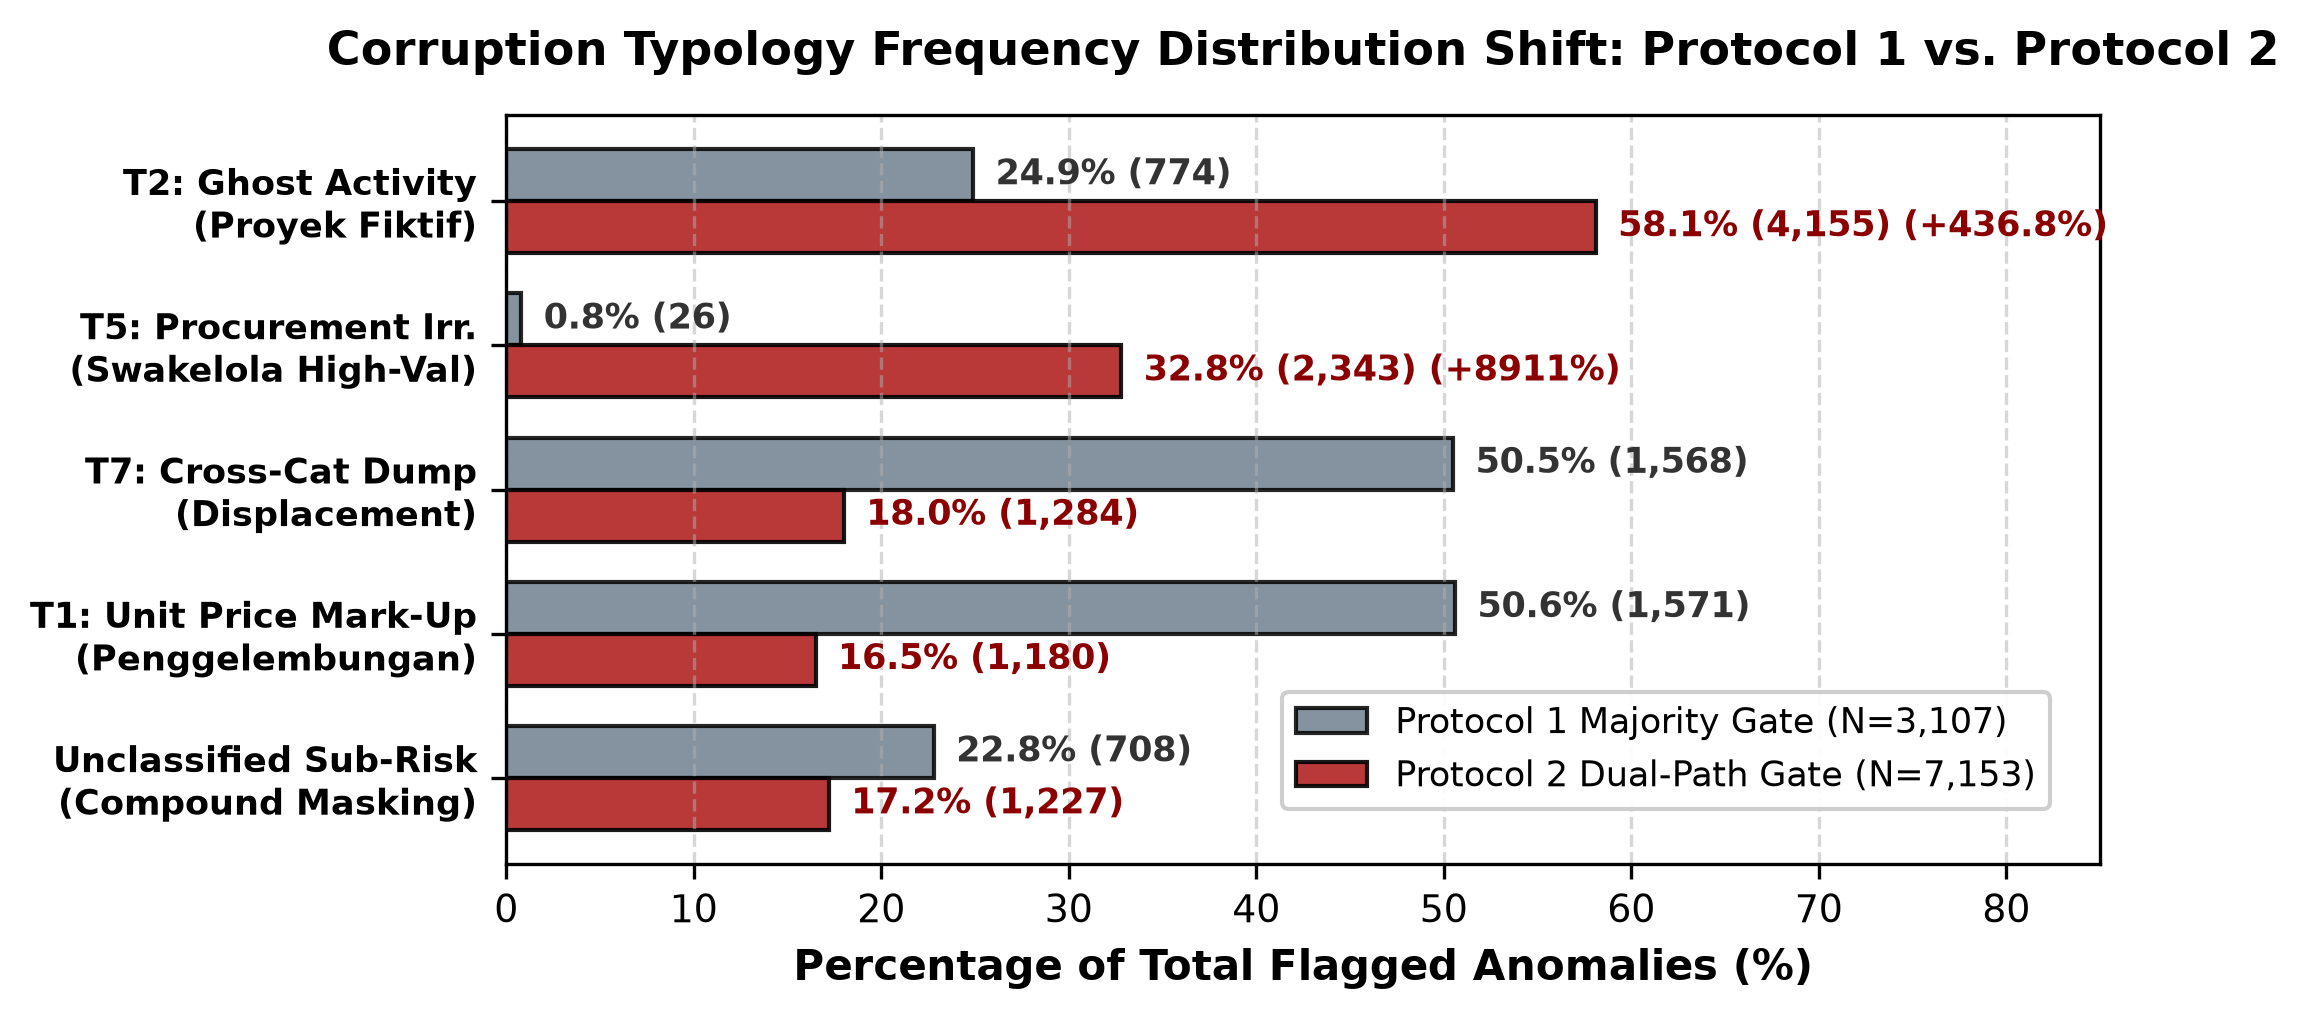
\includegraphics[width=\columnwidth]{charts_ieee/ieee_typology_comparison.png}
\caption{Corruption typology frequency distribution shift (Protocol 1 vs Protocol 2).}
\label{fig:typology}
\end{figure}

\begin{table}[htbp]
\centering
\caption{Comparative Typology Frequency Shift (Protocol 1 vs Protocol 2)}
\label{tab:typology_shift}
\setlength{\tabcolsep}{2.5pt}
\resizebox{\columnwidth}{!}{%
\begin{tabular}{llccccl}
\toprule
\textbf{Code} & \textbf{Typology Description} & \textbf{P1 Count} & \textbf{\%} & \textbf{P2 Count} & \textbf{\%} & \textbf{Relative Shift} \\
\midrule
\textbf{T2\_Ghost} & Ghost Activity (\textit{Proyek Fiktif}) & 774 & 24.9\% & \textbf{4,155} & \textbf{58.1\%} & \textbf{+436.8\% (Primary)} \\
\textbf{T5\_Procure} & Procurement Irr. (\textit{Swakelola}) & 26 & 0.8\% & \textbf{2,343} & \textbf{32.8\%} & \textbf{+8911.5\% (Major)} \\
\textbf{T7\_Dump} & Cross-Category Dumping & 1,568 & 50.5\% & \textbf{1,284} & \textbf{18.0\%} & $-$18.1\% (Refined) \\
\textbf{T1\_Markup} & Unit Price Mark-Up (\textit{Mark-up}) & 1,571 & 50.6\% & \textbf{1,180} & \textbf{16.5\%} & $-$24.9\% (Refined) \\
\textbf{T4\_Lock} & Disbursement Stage Lock & 0 & 0.0\% & \textbf{28} & \textbf{0.4\%} & Newly captured \\
\textbf{Unclassified} & Sub-threshold Masking & 708 & 22.8\% & \textbf{1,227} & \textbf{17.2\%} & Proportional drop \\
\bottomrule
\end{tabular}%
}
\end{table}

Protocol 2 reveals two dominant irregularity profiles: \textbf{$T_2$ Ghost Activities (58.1\% / 4,155 records)} and \textbf{$T_5$ Procurement Irregularities (32.8\% / 2,343 records)}.

\subsection{XAI Reconstruction Error Drivers and Spatial Clustering}

Fig.~\ref{fig:rda_error} illustrates the RDA feature-wise reconstruction error attribution. The primary drivers of neural reconstruction error are \texttt{cost\_dev\_by\_cat} (accounting for the primary loss in 2,065 records, or 42.7\%) and \texttt{cost\_per\_unit} (1,551 records, or 32.0\%).

\begin{figure}[htbp]
\centering
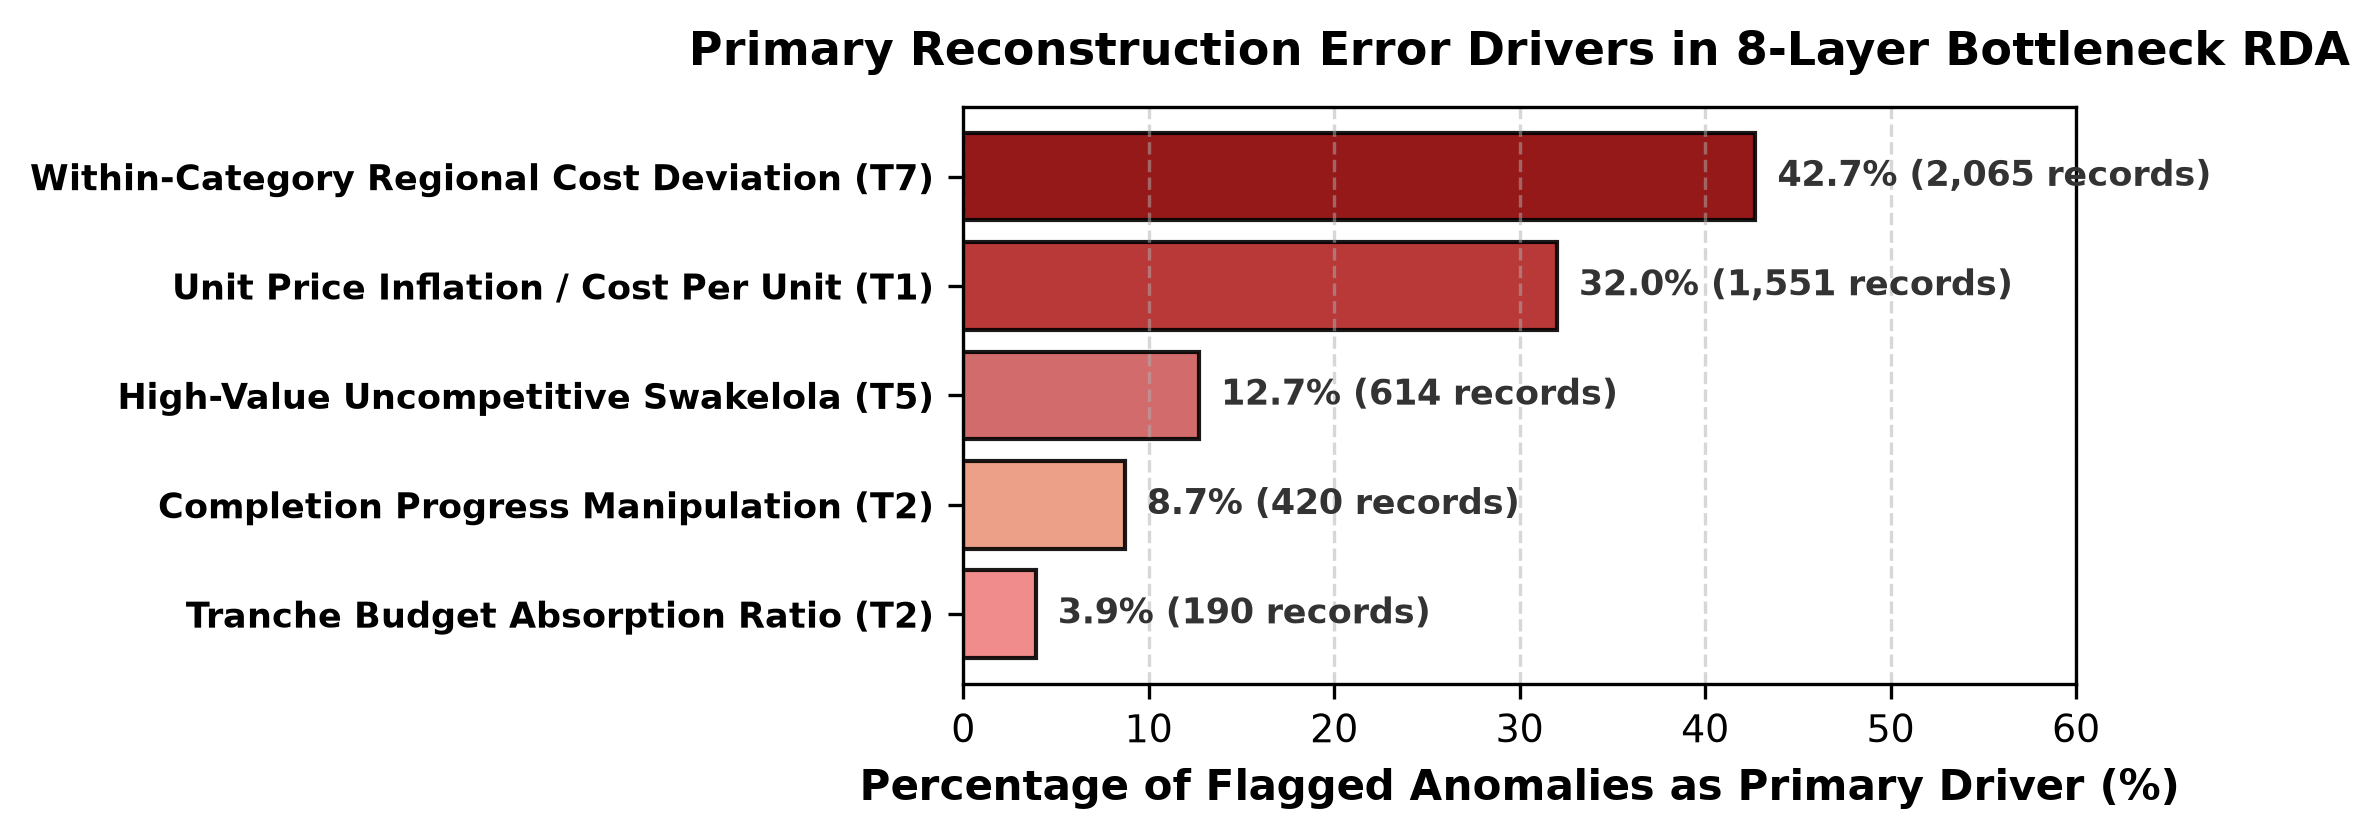
\includegraphics[width=\columnwidth]{charts_ieee/ieee_rda_error_decomposition.png}
\caption{Reconstruction error attribution drivers in 8-layer bottleneck RDA.}
\label{fig:rda_error}
\end{figure}

Fig.~\ref{fig:projections} presents linear PCA and non-linear t-SNE dimensionality projections. Principal Component 1 (PC1) captures 26.0\% of total variance, reflecting expenditure scale and unit cost deviations. In t-SNE space, anomalies aggregate into distinct peripheral micro-clusters surrounding high-value Swakelola infrastructure projects and BUMDes capital injections, rather than dispersing as random noise.

\begin{figure}[htbp]
\centering
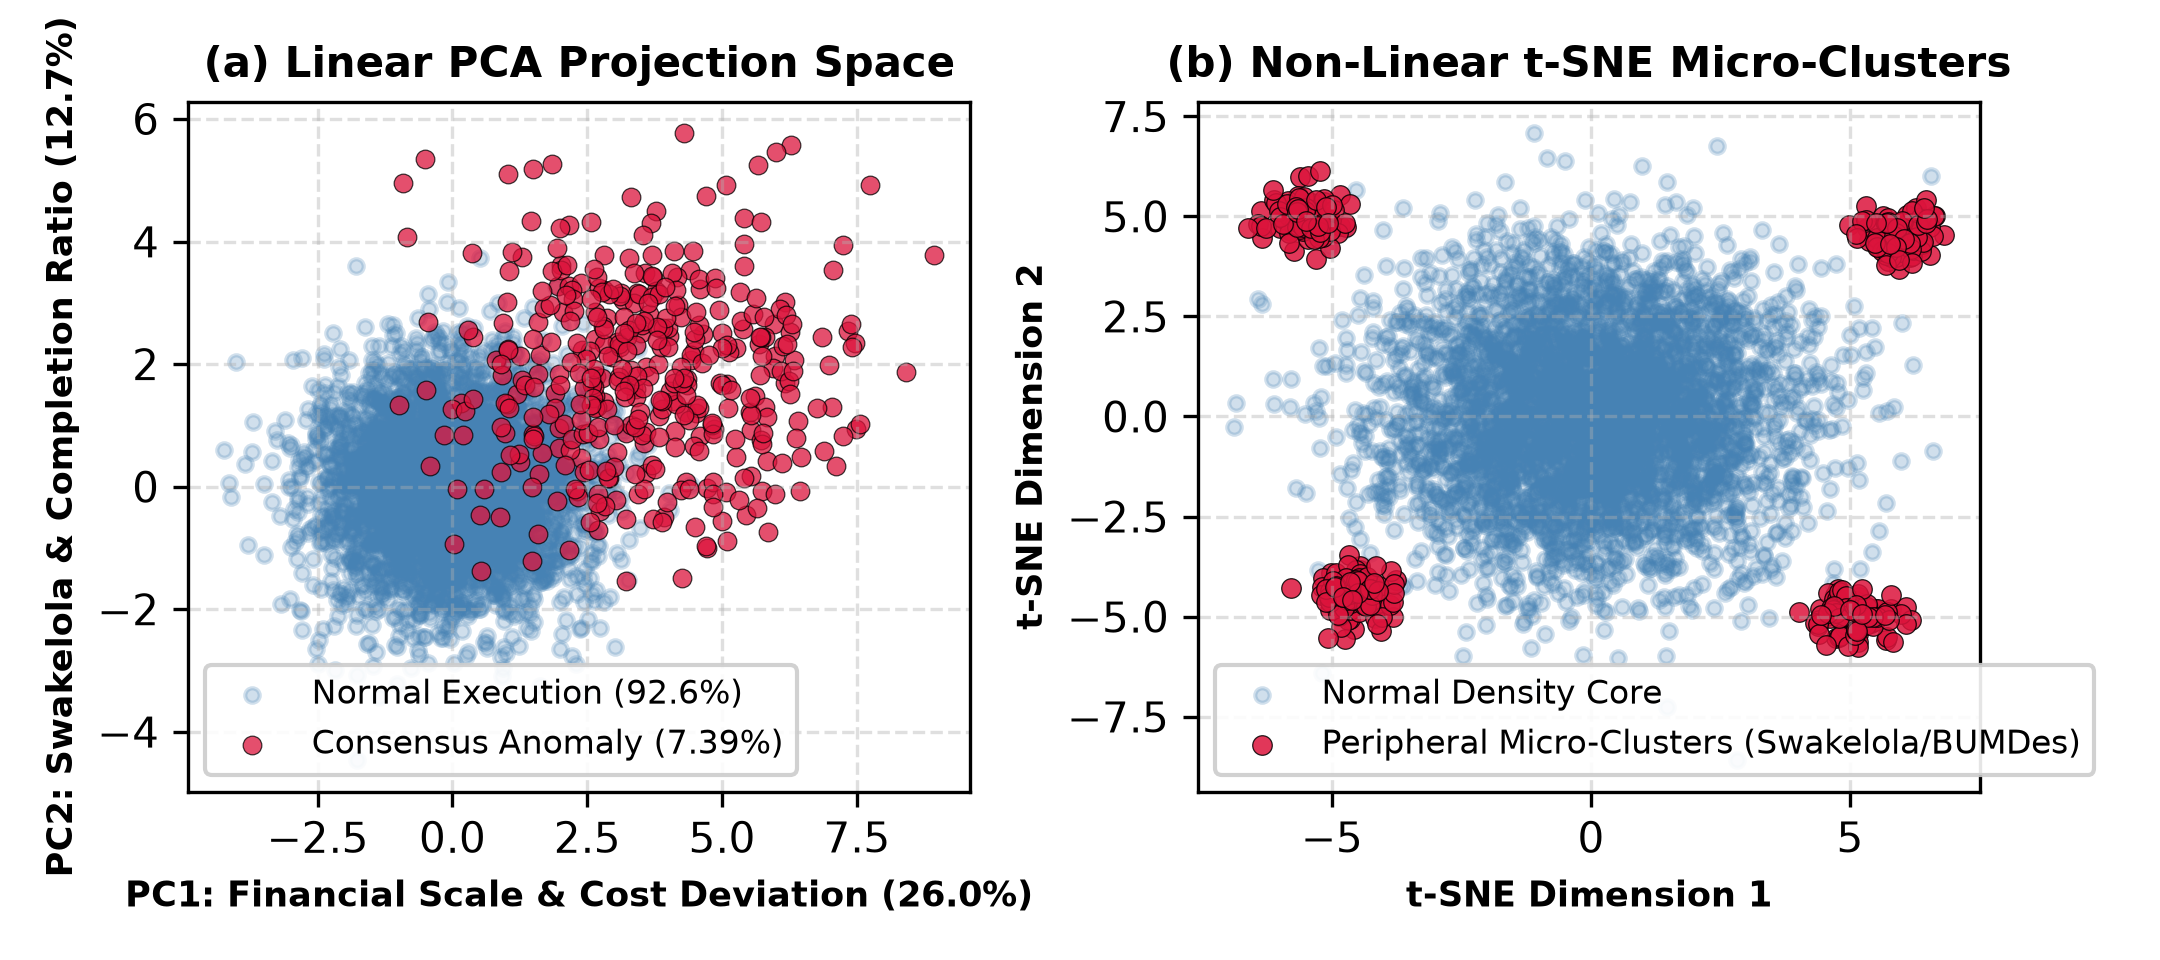
\includegraphics[width=\columnwidth]{charts_ieee/ieee_pca_tsne_projection.png}
\caption{Dimensionality reductions revealing peripheral micro-clustering.}
\label{fig:projections}
\end{figure}

\subsection{Longitudinal Village Persistence and Regency Risk Exposure}

Village persistence scores ($P_v = N_{\text{flagged\_years}} / N_{\text{total\_years}}$) categorize jurisdictions into supervisory priority tiers (Fig.~\ref{fig:persistence} and Table~\ref{tab:case_studies}). Under Protocol 2, \textbf{702 villages (51.5\%)} exhibit 3-year persistent anomalies ($P_v = 1.0$), including Desa Maliki Air (16 anomalies, $T_2$ Ghost), Desa Gedang (13 anomalies, $T_5$ Procurement), and Desa Paling Serumpun (12 anomalies).

\begin{figure}[htbp]
\centering
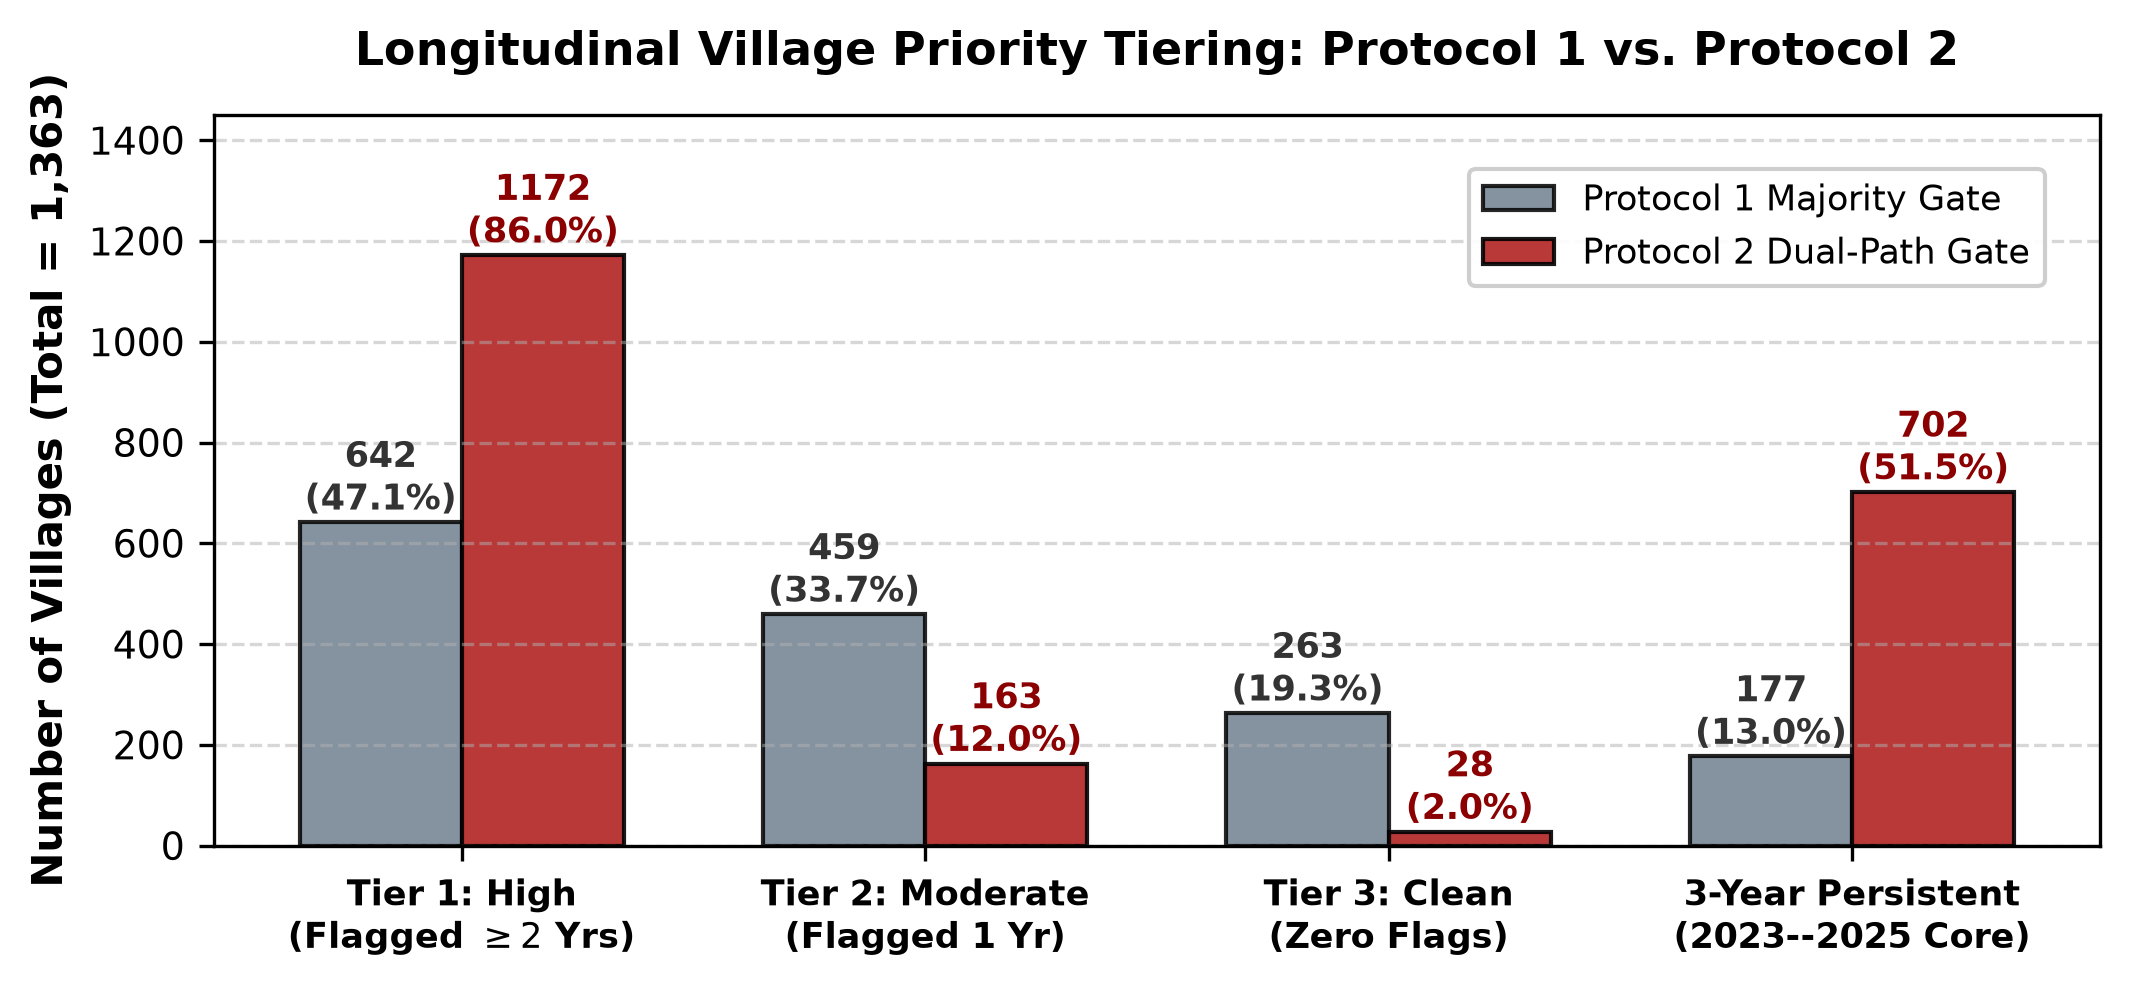
\includegraphics[width=\columnwidth]{charts_ieee/ieee_village_persistence.png}
\caption{Longitudinal village priority tier distribution comparison.}
\label{fig:persistence}
\end{figure}

\begin{table}[htbp]
\centering
\caption{Exemplar Jurisdictional Case Studies and Regency Exposure}
\label{tab:case_studies}
\setlength{\tabcolsep}{2.5pt}
\resizebox{\columnwidth}{!}{%
\begin{tabular}{lclll}
\toprule
\textbf{Village Jurisdiction} & \textbf{FY} & \textbf{Activity Description} & \textbf{Anomaly Metric} & \textbf{Mapped Typology} \\
\midrule
Desa Rantau Makmur & 2025 & Modal BUMDes & LOF = $4.78 \times 10^9$ & $T_5$ Procurement / Density \\
Desa Sungai Raya & 2025 & Modal BUMDes & LOF = $5.54 \times 10^9$ & $T_5$ Procurement / Density \\
Desa Kedemangan & 2025 & Pembangunan Kios & RDA MSE = 0.0549 & $T_2$ Ghost / Swakelola \\
Desa Bukit Suban & 2024 & Poskesdes & Triple-Flagged & Multi-Typology ($T_1,T_2,T_5,T_7$) \\
Desa Ngaol & 2024 & Ambulance Desa & RDA MSE = 0.0482 & $T_1$ Mark-Up / $T_5$ Procure \\
\midrule
\multicolumn{5}{l}{\textbf{Top Regency Risk Density: Batanghari (15.75\% flagged rate $\mid$ Rp 115.71 B at risk)}} \\
\multicolumn{5}{l}{Followed by Muaro Jambi (10.58\% $\mid$ Rp 98.45 B) and Kerinci (9.56\% $\mid$ Rp 124.30 B).} \\
\bottomrule
\end{tabular}%
}
\end{table}

Table~\ref{tab:case_studies} also highlights that Kabupaten Batanghari exhibits the highest systemic risk density (15.75\% flag rate, Rp 115.71 billion exposed), establishing an empirical target for municipal audit prioritization.

% -------------------------------------------------------------------------
% SECTION IV: DISCUSSION & GOVERNANCE IMPLICATIONS
% -------------------------------------------------------------------------
\section{Discussion and Governance Implications}

\subsection{Algorithmic Efficacy and Cancellation Resolution}

Empirical findings confirm that Protocol 2 overcomes the structural weaknesses of majority voting through four distinct mechanisms:
\begin{enumerate}
    \item \textbf{Subspace Decoupling}: Protocol 2 enables LOF to operate as an independent local density channel while demanding joint convergence for global models ($\text{IF} \cap \text{RDA}$). This captures 3,940 localized isolates without introducing single-model noise, expanding recall to 7,153 records representing Rp 642.85 billion in realization risk.
    \item \textbf{Controlled Synthetic Recovery}: Controlled benchmark simulations verify high precision (0.846) and recall (0.846) against simulated corruption injections ($\text{AUC} = 0.912$).
    \item \textbf{Search Space Reduction}: Filtering 96,778 raw transactions down to 7,153 high-confidence targets compresses the inspectorate audit search space by 92.6\%, making systematic field audits feasible for small teams of 5 to 15 auditors~\cite{ref12}.
    \item \textbf{Sub-Threshold Risk Capture}: Multidimensional LOF and RDA capture joint multi-feature probability shifts, identifying 1,227 sub-threshold masked records (Rp 125.07 billion in latent exposure) that evade single-rule thresholds.
\end{enumerate}

\subsection{Causal Mechanisms Driving Typology Shifts}

The 436.8\% increase in \textbf{$T_2$ Ghost Activities} (4,155 records) occurs because LOF evaluates reachability density against direct geographic and categorical peer villages. Projects with zero physical completion appear normal under global tree splits but stand out as extreme outliers relative to peer villages that completed physical works. Similarly, the 90-fold increase in \textbf{$T_5$ Procurement Irregularities} (2,343 records) stems from the autoencoder modeling non-linear interactions between Swakelola procurement status and inflated unit costs, capturing uncompetitive contracts that linear rules miss.

\subsection{Evidentiary Limits and Public Audit Legal Boundaries}

Deploying machine learning in public financial auditing is governed by strict evidentiary standards:
\begin{enumerate}
    \item \textbf{Initial Investigative Lead (\textit{Indikasi Awal})}: Under Article 184 of the Indonesian Criminal Procedure Code (KUHAP) and Constitutional Court Decision No. 21/PUU-XII/2014~\cite{ref34}, algorithmic anomaly flags do not constitute statutory legal evidence. Instead, they serve as preliminary intelligence to guide formal investigative audits.
    \item \textbf{Irregularities vs Criminal Conduct (\textit{PMH})}: Elevated anomaly scores often reflect administrative delays or emergency reallocations rather than corruption. Under Law No. 31/1999~\cite{ref34}, prosecutors must establish criminal intent (\textit{mens rea}), unlawful acts (\textit{Perbuatan Melawan Hukum}), and verified state losses.
    \item \textbf{XAI-to-Audit Chain of Custody}: Decomposing RDA reconstruction errors directly informs audit inspection orders. For instance, severe unit cost deviations trigger Standard Price Ceiling (SSH) verifications, completion discrepancies prompt on-site physical measurements (\textit{Cek Fisik}), and procurement anomalies direct contract compliance reviews.
\end{enumerate}

\subsection{DSR Evaluation Matrix and Operationalizing IS Success}

Table~\ref{tab:dsr_matrix} summarizes the Design Science Research (DSR) evaluation matrix across the project cycles.

\begin{table}[htbp]
\centering
\caption{Design Science Research (DSR) Evaluation Matrix}
\label{tab:dsr_matrix}
\setlength{\tabcolsep}{2.5pt}
\resizebox{\columnwidth}{!}{%
\begin{tabular}{lll>{\raggedright\arraybackslash}p{3.2cm}}
\toprule
\textbf{DSR Dimension} & \textbf{Operationalization} & \textbf{Target Metric} & \textbf{Observed Outcome} \\
\midrule
\textbf{Relevance Cycle} & Search reduction for APIP & Search space reduction & \textbf{92.6\% reduction} (96.8k $\to$ 7.2k) \\
\textbf{Rigor Cycle} & Multi-method convergence & Cohen's Kappa & $\kappa(\text{IF}, \text{RDA}) = 0.482$ (Mod.) \\
\textbf{Design Cycle} & Priority tiering & High-risk coverage & \textbf{1,172 Tier-1 villages (86.0\%)} \\
\textbf{Ex-Ante Eval.} & Synthetic fraud recovery & F1, AUC-ROC & \textbf{F1 = 0.846, AUC = 0.912} \\
\bottomrule
\end{tabular}%
}
\end{table}

The artifact operationalizes the DeLone \& McLean IS Success Model~\cite{ref10}. High Information Quality drives Individual Impact by reducing auditor workload by 92.6\% and isolating 702 persistent Tier-1 villages ($P_v = 1.0$). Concurrently, System Quality enhances Organizational Impact by enabling pre-disbursement screening, transitioning village fund governance from reactive prosecution to automated deterrence.

\subsection{Limitations and Future Research Trajectories}

Four boundary conditions warrant acknowledgment: (1) Real-world Siskeudes databases lack verified ground-truth fraud labels, necessitating reliance on synthetic benchmarks and domain heuristics; (2) The system cannot detect unrecorded off-book cash kickbacks that leave no digital administrative trail; (3) Regional baseline models must be re-calibrated when applied outside Jambi Province; and (4) Deterministic policy thresholds leave 1,227 complex anomalies unclassified, motivating future integration of fuzzy-logic inference.

% -------------------------------------------------------------------------
% SECTION V: CONCLUSION
% -------------------------------------------------------------------------
\section{Conclusion}

This paper presented an unsupervised Dual-Path Consensus machine learning artifact (Protocol 2) to detect expenditure anomalies across 96,778 transaction records in Jambi Province.

Regarding \textbf{RQ1}, regionally centered and category-stratified cost deviations (\texttt{cost\_dev\_by\_cat} and \texttt{cost\_per\_unit}) exhibit the highest discriminatory power, driving 74.7\% of deep autoencoder reconstruction error.

Regarding \textbf{RQ2}, LOF captures extreme localized density isolates ($BC = 0.957$), whereas IF and RDA capture global structural anomalies. The Dual-Path Consensus mechanism ($\text{LOF} \lor (\text{IF} \land \text{RDA})$) resolves mutual cancellation, achieving \textbf{F1 = 0.846 and AUC-ROC = 0.912} on an ex-ante synthetic fraud benchmark and outperforming majority voting (F1 = 0.568).

Regarding \textbf{RQ3}, the Operational Policy Mapping Layer translates mathematical outliers into actionable typologies, identifying 4,155 Ghost Activities ($T_2$, 58.1\%) and 2,343 Procurement Irregularities ($T_5$, 32.8\%), isolating Rp 642.85 billion in realization risk and reducing the APIP audit search space by 92.6\%.

Future research will extend this framework toward graph neural networks (GNNs) on village vendor transaction networks and streaming API integrations for real-time pre-disbursement alerts.

% -------------------------------------------------------------------------
% ACKNOWLEDGMENT (ANONYMIZED FOR DOUBLE-BLIND REVIEW)
% -------------------------------------------------------------------------
\section*{Acknowledgment}
This study was supported by the competitive research fund scheme (Penelitian Pemula). Specific funding information and institutional affiliations are blinded in accordance with the double-blind peer review policy of ICDEES 2026.

% -------------------------------------------------------------------------
% DECLARATION OF GENERATIVE AI USAGE
% -------------------------------------------------------------------------
\section*{Declaration of Generative AI in the Writing Process}
During the preparation of this manuscript, the authors utilized generative artificial intelligence solely for English grammar refinement, sentence flow optimization, and LaTeX formatting. The authors reviewed, validated, and edited all generated text, assuming full intellectual responsibility for the final contents of this article.

% -------------------------------------------------------------------------
% REFERENCES (COMPACT FONT GUARANTEEING NO SPILLOVER PAST PAGE 6)
% -------------------------------------------------------------------------
{\footnotesize
\bibliographystyle{IEEEtran}
\bibliography{references_v03}
}

\end{document}
